\documentclass[preview,tikz,convert={outext=.svg,command=\unexpanded{pdf2svg \infile\space\outfile}},multi=false]{standalone}[2022/10/10]
%\usetikzlibrary{...}% tikz package already loaded by 'tikz' option
\usepackage[european,siunitx]{circuitikz}
\usetikzlibrary[circuits.plc.ladder]
\makeatletter
\begin{document}
    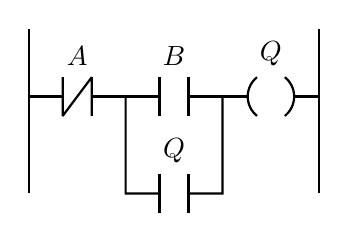
\begin{tikzpicture}[circuit plc ladder,thick,ladderrungsep=0.8]
        \draw(0,0)
        to [contact NC={info={$A$},name=ca}] ++(1,0)
        to [contact NO={info={$B$},name=ca}] ++(1,0)
        to [coil={info={$Q$}}] ++(1,0) coordinate(laddertopright);
        \draw(1, 0)
        -- ++(0,-1)
        to [contact NO={info={$Q$},name=ca}] ++(1,0) -- +(0,1);
        \ladderrungend{1}
        \ladderpowerrails
    \end{tikzpicture}
\end{document}